%%%%%%%%%%%%%%%%%%%%%%%%%%%%%%%%%%%%%%%%%
% Masters/Doctoral Thesis 
% LaTeX Template
% Version 2.5 (27/8/17)
%
% This template was downloaded from:
% http://www.LaTeXTemplates.com
%
% Version 2.x major modifications by:
% Vel (vel@latextemplates.com)
%
% This template is based on a template by:
% Steve Gunn (http://users.ecs.soton.ac.uk/srg/softwaretools/document/templates/)
% Sunil Patel (http://www.sunilpatel.co.uk/thesis-template/)
%
% Template license:
% CC BY-NC-SA 3.0 (http://creativecommons.org/licenses/by-nc-sa/3.0/)
%
%%%%%%%%%%%%%%%%%%%%%%%%%%%%%%%%%%%%%%%%%

%----------------------------------------------------------------------------------------
%	PACKAGES AND OTHER DOCUMENT CONFIGURATIONS
%----------------------------------------------------------------------------------------

\documentclass[
11pt, % The default document font size, options: 10pt, 11pt, 12pt
oneside, % Two side (alternating margins) for binding by default, uncomment to switch to one side
english, % ngerman for German
onehalfspacing,%singlespacing, % Single line spacing, alternatives: onehalfspacing or doublespacing
%draft, % Uncomment to enable draft mode (no pictures, no links, overfull hboxes indicated)
%nolistspacing, % If the document is onehalfspacing or doublespacing, uncomment this to set spacing in lists to single
%liststotoc, % Uncomment to add the list of figures/tables/etc to the table of contents
%toctotoc, % Uncomment to add the main table of contents to the table of contents
%parskip, % Uncomment to add space between paragraphs
%nohyperref, % Uncomment to not load the hyperref package
headsepline, % Uncomment to get a line under the header
%chapterinoneline, % Uncomment to place the chapter title next to the number on one line
%consistentlayout, % Uncomment to change the layout of the declaration, abstract and acknowledgements pages to match the default layout
]{BachelorThesis} % The class file specifying the document structure
\usepackage[utf8]{inputenc} % Required for inputting international characters
\usepackage[T1]{fontenc} % Output font encoding for international characters
\usepackage{mathpazo} % Use the Palatino font by default
\usepackage[backend=bibtex,style=numeric,citestyle=numeric,natbib=true]{biblatex} % Use the bibtex backend with the authoryear citation style (which resembles APA)
\usepackage[autostyle=true]{csquotes} % Required to generate language-dependent quotes in the bibliography
\usepackage{enumitem} 
\usepackage{listings}
\usepackage{graphicx}
\usepackage{xspace}
\usepackage[export]{adjustbox}
\usepackage{xcolor}
\usepackage{amsmath}
\usepackage[font={small}]{caption}
\usepackage{varwidth}	
\usepackage{supertabular}
%\usepackage[caption=false]{subfig}
\usepackage{float}
%\usepackage{cite}
\usepackage{amsmath,amssymb,amsfonts}
\usepackage{algorithmic}
\usepackage{graphicx}
\usepackage{textcomp}
\usepackage{xcolor, colortbl}
\usepackage{booktabs}
\usepackage{multirow}
\usepackage{xspace}
\usepackage{caption}
\usepackage{multicol}
\usepackage{subcaption}
\usepackage{footnote}
\usepackage{url}
\usepackage{gitinfo2}
\usepackage{tcolorbox}
\usepackage[para]{footmisc}
\usepackage{array,ragged2e}

\usepackage{listings}

\usepackage{amssymb}
\usepackage{ifthen}


%%%%%%%%%% main %%%%%%%%%%
\newcommand{\ie}{\emph{i.e.,}\xspace}
\newcommand{\eg}{\emph{e.g.,}\xspace}
\newcommand{\etc}{etc.\xspace}
\newcommand{\etal}{\emph{et~al.}\xspace}
\newcommand{\secref}[1]{Section~\ref{#1}\xspace}
\newcommand{\capref}[1]{\textit{Chapter~\ref{#1}\xspace}}
\newcommand{\figref}[1]{Fig.~\ref{#1}\xspace}
\newcommand{\listref}[1]{Listing~\ref{#1}\xspace}
\newcommand{\tabref}[1]{Table~\ref{#1}\xspace}
\newcommand{\tool}[1]{{\sc #1}\xspace}
\newcommand{\commitref}[1]{\texttt{#1}}

%Experiement
\newcommand{\totalCommits}{19,603,736\xspace}
\newcommand{\validated}{3,585\xspace}
\newcommand{\finalInstances}{1,930\xspace}
\newcommand{\finalInstancesPercent}{55.6\%\xspace}
\newcommand{\finalInstancesIssues}{224\xspace}
\newcommand{\finalInstancesIssuesPercent}{11.2\%\xspace}
\newcommand{\oracle}{1,115\xspace}
\newcommand{\oracleWithIssue}{129\xspace}

% %%%%%%%%%%%%%%%%%%%%%%%%%%%%
% UTILS
% %%%%%%%%%%%%%%%%%%%%%%%%%%%%

\newcommand{\RQ}[1]{RQ$_{#1}$\xspace}

\newcommand{\ourtool}{\textsc{ARGOS}\xspace}
\newcommand{\ourtoolfullname}{{utterAnces vaRiant Generator for vOcal user interfaceS}\xspace}

\newcommand{\finetuningsample}{{371}\xspace}
\newcommand{\similaritythreshold}{\textit{0.75}\xspace}

\newcommand{\samplerqoneour}{{327}\xspace}
\newcommand{\totgeneratedour}{{2186}\xspace}
\newcommand{\anomaliesour}{{363}\xspace}
\newcommand{\bugsour}{{167}\xspace}

\newcommand{\samplerqoneamazon}{{246}\xspace}
\newcommand{\totgeneratedamazon}{{680}\xspace}
\newcommand{\anomaliesamazon}{{124}\xspace}
\newcommand{\bugsamazon}{{43}\xspace}
\newboolean{showcomments}


\setboolean{showcomments}{true}

\ifthenelse{\boolean{showcomments}}
{\newcommand{\nb}[2]{
		\fbox{\bfseries\sffamily\scriptsize#1}
		{\sf\small$\blacktriangleright$\textit{#2}$\blacktriangleleft$}
	}
}
{\newcommand{\nb}[2]{}
}

\newcommand{\bszz}{\textsc{B-SZZ}\xspace}
\newcommand{\agszz}{\textsc{AG-SZZ}\xspace}
\newcommand{\djszz}{\textsc{DJ-SZZ}\xspace}
\newcommand{\rszz}{\textsc{R-SZZ}\xspace}
\newcommand{\lszz}{\textsc{L-SZZ}\xspace}
\newcommand{\maszz}{\textsc{MA-SZZ}\xspace}
\newcommand{\raszz}{\textsc{RA-SZZ}\xspace}
\newcommand{\raszzs}{\textsc{RA-SZZ\textsuperscript{*}}\xspace}

\newcommand{\justcitebszz} {\cite{sliwerski2005changes}\xspace}
\newcommand{\justciteagszz}{\cite{kim2006automatic}\xspace}
\newcommand{\justcitedjszz}{\cite{williams2008szz}\xspace}
\newcommand{\justciterlszz}{\cite{davies2014comparing}\xspace}
\newcommand{\justcitemaszz}{\cite{da2016framework}\xspace}
\newcommand{\justciteraszz}{\cite{neto2018impact}\xspace}
\newcommand{\justciteraszzs}{\cite{neto2019revisiting}\xspace}

\newcommand{\citeallszz}{\cite{sliwerski2005changes, kim2006automatic, williams2008szz, davies2014comparing, da2016framework, neto2018impact, neto2019revisiting}\xspace}
\newcommand{\citeallimprovedszz}{\cite{kim2006automatic, williams2008szz, davies2014comparing, da2016framework, neto2018impact, neto2019revisiting}\xspace}

\newcommand{\citebszz}{\'Sliwerski \etal \cite{sliwerski2005changes}\xspace}
\newcommand{\citeagszz}{Kim \etal \cite{kim2006automatic}\xspace }
\newcommand{\citedjszz}{Williams and Spacco \cite{williams2008szz}\xspace}
\newcommand{\citerlszz}{Davies \etal \cite{davies2014comparing}\xspace}
\newcommand{\citemaszz}{da Costa \etal \cite{da2016framework}\xspace}
\newcommand{\citeraszz}{Neto \etal \cite{neto2018impact}\xspace}
\newcommand{\citeraszzs}{Neto \etal \cite{neto2019revisiting}\xspace}


%%%%%%%%%% introduction %%%%%%%%%%
\newcommand{\manual}{Manually defined (researchers)\xspace}
\newcommand{\bszzuses}{\cite{palomba2018diffuseness, pascarella2019fine, ccaglayan2016effect, wen2016locus, posnett2013dual, kim2008classifying, tan2015online, kononenko2015investigating, wehaibi2016examining, lenarduzzi2020sonarqube}}
\newcommand{\agszzuses}{\cite{tufano2017empirical, bernardi2018relation, hata2012bug, rahman2011bugcache, eyolfson2014correlations, misirli2016studying, canfora2011long, prechelt2014software, bird2009fair}}
\newcommand{\djszzuses}{\cite{marinescu2014covrig, borg2019szz, bavota2015four, toth2016public, fan2019impact, karampatsis2019often, rodriguez2020bugs, rodriguez2018reproducibility}}
\newcommand{\rlszzuses}{\cite{da2016framework}}
\newcommand{\maszzuses}{\cite{fan2019impact, neto2018impact, neto2019revisiting, tu2020better, aman2019empirical, chen2019extracting}}
\newcommand{\raszzuses}{\cite{fan2019impact, neto2018impact, yan2020just}}
\newcommand{\raszzsuses}{None}


%%%%%%%%%% deisgn %%%%%%%%%%
\newcommand{\rqOne}{How do different variants of SZZ perform in identifying bug-inducing changes?}
\newcommand{\oracleAllDataset}{$\mathit{oracle}_{\mathit{all}}$\xspace}
\newcommand{\oracleIssueDataset}{$\mathit{oracle}_{\mathit{issues}}$\space}
\newcommand{\oracleAllDatasetJava}{$\mathit{oracle}_{\mathit{all}}^{J}$\xspace}
\newcommand{\oracleIssueDatasetJava}{$\mathit{oracle}_{\mathit{issues}}^{J}$\space}

\definecolor{Gray}{gray}{0.9}

\lstset{
	language=C,
	%basicstyle=\small,
	breaklines=true
}

\def\BibTeX{{\rm B\kern-.05em{\sc i\kern-.025em b}\kern-.08em
		T\kern-.1667em\lower.7ex\hbox{E}\kern-.125emX}}


\addbibresource{references.bib} % The filename of the bibliography

\graphicspath{
	{Figures/}
}

\newcommand\TODO[1]{\textcolor{red}{\nb{TODO}{#1}}}

\newenvironment{blueparagraph}{\par\color{blue}}{\par}
\newenvironment{nscenter}
{\parskip=0pt\par\nopagebreak\centering}
{\par\noindent\ignorespacesafterend}

%----------------------------------------------------------------------------------------
%	MARGIN SETTINGS
%----------------------------------------------------------------------------------------

\geometry{
	paper=a4paper, % Change to letterpaper for US letter
	inner=2.5cm, % Inner margin
	outer=3.8cm, % Outer margin
	bindingoffset=.5cm, % Binding offset
	top=1.5cm, % Top margin
	bottom=1.5cm, % Bottom margin
	%showframe, % Uncomment to show how the type block is set on the page
}

%----------------------------------------------------------------------------------------
%	THESIS INFORMATION
%----------------------------------------------------------------------------------------

\thesistitle{A Fine-Grained Analysis of Comments Quality in Code-Related Datasets} % Your thesis title, this is used in the title and abstract, print it elsewhere with \ttitle
\supervisor{Prof. Simone \textsc{Scalabrino}} % Your supervisor's name, this is used in the title page, print it elsewhere with \supname
\examiner{} % Your examiner's name, this is not currently used anywhere in the template, print it elsewhere with \examname
\degree{Informatica} % Your degree name, this is used in the title page and abstract, print it elsewhere with \degreename
\author{Angelo \textsc{Trotta}} % Your name, this is used in the title page and abstract, print it elsewhere with \authorname
\addresses{} % Your address, this is not currently used anywhere in the template, print it elsewhere with \addressname

\subject{Automated Software Delivery} % Your subject area, this is not currently used anywhere in the template, print it elsewhere with \subjectname
\keywords{} % Keywords for your thesis, this is not currently used anywhere in the template, print it elsewhere with \keywordnames
\university{\href{https://www.unimol.it/}{Università degli Studi del Molise}} % Your university's name and URL, this is used in the title page and abstract, print it elsewhere with \univname
\department{\href{http://dipbioter.unimol.it/}{Dipartimento di Bioscienze e Territorio}} % Your department's name and URL, this is used in the title page and abstract, print it elsewhere with \deptname
%\faculty{\href{http://faculty.university.com}{Faculty Name}} % Your faculty's name and URL, this is used in the title page and abstract, print it elsewhere with \facname

\AtBeginDocument{
	\hypersetup{pdftitle=\ttitle} % Set the PDF's title to your title
	\hypersetup{pdfauthor=\authorname} % Set the PDF's author to your name
	\hypersetup{pdfkeywords=\keywordnames} % Set the PDF's keywords to your keywords
}


\begin{document}
	\renewenvironment{abstract} 
	
	\frontmatter % Use roman page numbering style (i, ii, iii, iv...) for the pre-content pages
	
	\pagestyle{plain} % Default to the plain heading style until the thesis style is called for the body content
	
	%----------------------------------------------------------------------------------------
	%	TITLE PAGE
	%----------------------------------------------------------------------------------------
	
	\begin{titlepage}
		\begin{center}
			
			
\includegraphics[width=0.35\textwidth]{figs/logo} % University/department logo - uncomment to place it
			
			\vspace{0.75cm}

			{\scshape\huge \univname\par}\vspace{0.15cm} % University name
			
			{\scshape\Large \deptname\par}\vspace{1cm} % University name
			
			\text{\Large Corso di Laurea in}\\[0.05cm]
			
			\textsc{\Large \degreename}\\[1cm]
			
			\text{\Large Tesi in}\\[0.05cm]
			
			\textsc{\Large \subjectname}\\[1cm] % Thesis type
			
			%\HRule \\[0.4cm] % Horizontal line
			{\huge \bfseries \ttitle\par}\vspace{1.5cm} % Thesis title
			%\HRule \\[1.5cm] % Horizontal line
			
			\begin{minipage}[t]{0.95\textwidth}
					\Large \emph{Candidato:} \\
					{\authorname}\\[0.1cm] % Author name - remove the \href bracket to remove the link
					%\href bracket to remove the link 
					\emph{Matricola:} {171874} 
			\end{minipage}
			\begin{minipage}[t]{0.95\textwidth}
				\begin{flushright} \Large
					\emph{Relatore:}\\
					\href{https://dibt.unimol.it/staff/sscalabrino/home/}{\supname} % Supervisor name - remove the \href bracket to remove the link
					\begin{flushright} \Large
						\emph{Co-Relatore:}\\
						\href{https://scholar.google.com/citations?user=AdVTnyQAAAAJ&hl=it}{Dr. Antonio \textsc{Vitale}} % Correlator name 
					\end{flushright} 
				\end{flushright}
				%\begin{flushright} \large
				%\emph{Co-Supervisor:} \\
				%%\href{https://www.inf.usi.ch/faculty/bavota/}{Dr. Simone \textsc{Scalabrino}} \\% Correlator name 
				%\href{https://dibt.unimol.it/staff/sscalabrino/home/}{Dr. Giovanni \textsc{Rosa}} % Correlator name 
				
				%\end{flushright}
			\end{minipage}\\[1.5cm]
			
			\vfill
			
			\centerline{\Large Anno Accademico 2023/2024}
		\end{center}
	\end{titlepage}
	
%----------------------------------------------------------------------------------------
%	BLANK PAGE
%----------------------------------------------------------------------------------------
\pagenumbering{gobble}
%\dedicatory{\textit{Thanks}}
\newpage

%----------------------------------------------------------------------------------------
%	LIST OF CONTENTS/FIGURES/TABLES PAGES
%----------------------------------------------------------------------------------------
\newpage\pagenumbering{Roman}

\tableofcontents % Prints the main table of contents
\listoffigures % Prints the list of figures

%\listoftables % Prints the list of tables

%----------------------------------------------------------------------------------------
%	THESIS CONTENT - CHAPTERS
%----------------------------------------------------------------------------------------

\mainmatter % Begin numeric (1,2,3...) page numbering

\pagestyle{thesis} % Return the page headers back to the "thesis" style

% Include the chapters of the thesis as separate files from the Chapters folder
% Uncomment the lines as you write the chapters

% Chapter 1

\chapter{Introduction} % Main chapter title

\label{Chapter1} % For referencing the chapter elsewhere, use \ref{Chapter1} 

%----------------------------------------------------------------------------------------

% Define some commands to keep the formatting separated from the content 
\newcommand{\keyword}[1]{\textbf{#1}}
\newcommand{\tabhead}[1]{\textbf{#1}}
\newcommand{\code}[1]{\texttt{#1}}
\newcommand{\file}[1]{\texttt{\bfseries#1}}
\newcommand{\option}[1]{\texttt{\itshape#1}}

%----------------------------------------------------------------------------------------

\section{Application Context} In the field of software development, the practice of commenting written code is widely recognized, as it serves multiple functions in the application and maintenance of software systems.

\noindent Comments are non-executable statements embedded within code to provide explanations, clarify intent, and guide future developers or collaborators who may interact with the codebase. While it may seem an easy job to write comments at first glance, general principles and good practices \cite{commentingPrinciples} are often overlooked.
While comments do not affect the program’s execution, they play an essential role in enhancing \textbf{code readability} \cite{codeReadability}, \textbf{maintainability} \cite{codeMaintainability}, and \textbf{collaboration}, which are critical to software development as a whole in both small teams and large organizations.

\noindent When writing comments, it is important to strike a balance in their length, ensuring they are neither too brief nor overly detailed. Comments should be concise yet informative, providing enough context without overwhelming the reader with unnecessary details.
For documentation comments, developers must adhere to the specific syntax and formatting rules of the programming language being used, particularly when it comes to annotations and tags, to ensure proper integration with documentation tools.
Technical comments added during development should be revised or removed when they become obsolete. Outdated or irrelevant comments can lead to confusion and misinterpretation, detracting from code clarity rather than enhancing it.
Additionally, comments should avoid posing questions, as their primary function is to clarify and guide, not to introduce uncertainty. Lastly, comments must not be left empty, as they serve no purpose and only add clutter to the codebase.

\noindent Given these premises, it is therefore imperative to make sure comments are verified to be correctly written, with as high quality as possible.


\section{Motivation and Objectives}
Developing a comment analysis system \cite{commentAnalysis} is a challenging task, as it requires a deep understanding of the rules governing the programming language in which the code is written, alongside ensuring computational accuracy and efficiency when processing comment data.

\noindent Additionally, the content of comments can often be complex or ambiguous, making it difficult for automated heuristics to handle certain scenarios correctly. In such cases, manual review may be necessary to address edge cases or interpret unclear comments.
Therefore, it is crucial to ensure that the system is robust and effective for the vast majority of use cases, while acknowledging that some instances may require additional intervention.

\noindent The objective of this work is to define an approach for the automatic analysis of large code-related datasets, aiming to identify comments that fail to meet an adequate level of quality based on the following criteria:
\begin{itemize}
	\item \textbf{Empty comments}: as previously mentioned, empty comments serve no purpose and should be flagged immediately during analysis, as they offer no value or clarity to the code.
	\item \textbf{Comments asking questions}: whether direct or implied (with or without a question mark), questions contradict the purpose of comments—providing clear, definitive information to the reader.
	\item \textbf{Short comments}: they lack sufficient information to explain the code adequately. Their brevity prevents them from offering the necessary context to help readers understand the functionality or purpose of the code.
	\item \textbf{Long comments}: conversely, they tend to provide excessive detail, overwhelming the reader with unnecessary information. This can result in confusion and misinterpretation, as too much data often obscures the main point.
	\item \textbf{Comments under development}: these are highly technical, often temporary comments relevant only to developers actively working on the project. Such comments need regular updates or removal once they no longer reflect the current state of the system.
	\item \textbf{Incomplete comments}: they clearly indicate missing information, either in terms of sentence structure or overall completeness. They fail to fully communicate the intended message or explanation, leaving the reader with gaps in understanding.
	\item \textbf{Uneven comments format}: with irregular structure or formatting, they contribute to clutter and hinder readability. A lack of consistency in style makes comments harder to follow and increases the difficulty of understanding and maintaining the code. Comments should adhere to a uniform format to ensure clarity and ease of use.
\end{itemize}

\section{Results}
Comments play an important role in improving the performance of code completion models \cite{vandam2023}.
The presence of multi-line comments was found to significantly enhance the performance of pre-trained language models like \textit{UniXcoder}, \textit{CodeGPT}, and \textit{InCoder}. The study, led by \href{https://arxiv.org/search/cs?searchtype=author&query=van+Dam,+T}{\textit{Tim van Dam}}, \href{https://arxiv.org/search/cs?searchtype=author&query=Izadi,+M}{\textit{Maliheh Izadi}} and \href{https://arxiv.org/search/cs?searchtype=author&query=van+Deursen,+A}{\textit{Arie van Deursen}} suggests that natural language descriptions embedded in multi-line comments contribute to the models' ability to understand and complete code, making these comments valuable in datasets used for training and evaluating code-related tasks.

\noindent The paper of \textit{Are We Building On The Rock?} \cite{buildingRock} notes how comments are also important in the context of code summarization tasks.
High-quality comments enhance the ability of code summarization models to generate accurate and useful descriptions of source code. However, it's also noted how noisy or poor-quality comments can significantly reduce the effectiveness of these models.

\noindent Using the approach described above, our goal is to obtain a reliable set of comment indices for each category from an input dataset. To enhance the quality of the output, we apply natural language processing (NLP) techniques in certain cases, ensuring the accuracy and relevance of the results. Additionally, we conducted an empirical study to evaluate the effectiveness of our approach on a sample dataset consisting of manually selected instances.

\noindent We compared the automated results produced by our tool with a thorough manual analysis of the same sample. The comparison aimed to ensure that the error rate of our tool remained within a ±5\% margin. Finally, we identified the key limitations of our approach and provided recommendations for future research and improvements. The main contributions of this paper can be summarized as follows:
\begin{itemize}
    \item We proposed an analysis tool for automatic detection of lack of comments quality, evaluated under different criteria;
    \item We used a set of carefully selected datasets to train our approach;
    \item We defined case-study samples from selected datasets to verify the correctness of our approach.
\end{itemize}

\section{Thesis Structure and Organization}
The next chapters of this thesis are:

\begin{itemize}
\item \textit{Chapter 2}: presents background and related works.
\item \textit{Chapter 3}: presents our heuristics for detecting lack of comments quality for each category.
\item \textit{Chapter 4}: presents the empirical study conducted to validate the
defined heuristic.
\item \textit{Chapter 5}: describes the building process of our tool.
\item \textit{Chapter 6}: concludes this thesis and provides directions for future
works.

\end{itemize}
% Chapter 2

\chapter{Background and Related Work} % Main chapter title

\label{Chapter2} 

\section{Comments Quality}
Comment quality refers to how effectively developers convey information about the tasks the code fulfills. Writing clear, helpful comments is essential for maintaining software over time. Source code without adequate comments becomes difficult to maintain, as developers may struggle to make changes without fully understanding its purpose or functionality. High-quality comments should be readable, well-organized, syntactically accurate, and logically clear. They must cater to both experienced and inexperienced developers, ensuring that the code is accessible to anyone who works on it.

\noindent There are several practices that can undermine or improve comments quality. For example, when dealing with long and complex methods, the accompanying comment should be concise, straightforward, and focus on key points. Providing examples where relevant can enhance clarity. Comments should also adhere to proper indentation and line-break styles, as inconsistent formatting or excessive spacing can cause confusion and reduce readability.

\noindent Issues can arise when outdated or deprecated methods are left commented out within the code, often cluttering more useful, current comments. If a comment is intended as documentation, it should match the method’s parameters and return types to ensure accuracy and relevance.

\noindent Ideally, comments should only be added when necessary. When included, they should provide a description that is both concise and cohesive, avoiding redundancy or excessive detail. Inline comments within methods that explain actions as they occur are particularly useful, as they help guide readers through the code step by step, making it easier to follow and understand.

\section{Comments Quality Analysis}
Several studies have been conducted to analyze the quality of comments across various datasets. One such approach, presented by \textit{Khamis et al.} \cite{javadocMiner}, offers an effective and automated approach for evaluating the quality of inline documentation using a set of heuristics. Their method assesses both the linguistic quality of comments and the consistency between source code and its corresponding documentation. The researchers applied their approach to different modules of two open-source applications, \textit{ArgoUML} and \textit{Eclipse}, comparing the analysis results with bug reports from the individual modules. This comparison aimed to uncover potential connections between documentation quality and overall code quality, shedding light on how well-maintained comments may influence software reliability.

\noindent \textit{Steidl et al.} \cite{steidl2013} proposed a model for evaluating comment quality based on different comment categories. The researchers used machine learning techniques to categorize comments from \textit{Java} and \textit{C/C++} programs, allowing for a more structured analysis of comment quality. By applying metrics tailored to specific comment categories, they were able to effectively assess key quality aspects within the model, providing valuable insights into the strengths and weaknesses of code comments in these programming languages.

\noindent \textit{Lin Tan} \cite{TAN2015493} highlighted the wealth of information contained in code comments and how this can be used to enhance software maintainability and reliability. He conducted a detailed study and analysis of both free-form and semistructured comments, demonstrating their potential to improve the overall quality and robustness of software systems.

\noindent \textit{Pooja Rani} \cite{Rani2021} addressed the problem of evaluating code comments, exploring comment quality assessment from three perspectives:
\begin{itemize}
	\item \textbf{Developer Concerns}: the study investigates what developers ask about commenting practices, identifying a taxonomy of common concerns and challenges faced by developers when writing or generating code comments.
	\item \textbf{Information Types}: it categorizes the various types of information embedded in class comments across different programming languages. An automated classification method using machine learning and NLP techniques is proposed to identify these comment types.
	\item \textbf{Research Support}: a systematic literature review was conducted to compile a taxonomy of comment quality attributes and metrics, helping to develop a unified approach for assessing the quality of code comments based on empirical data.
\end{itemize}

\noindent \textit{Hao He} \cite{HaoHe19} investigated the patterns and practices of code commenting across different programming languages and project types. By analyzing 150 popular projects in five programming languages (\textit{JavaScript}, \textit{Java}, \textit{C++}, \textit{Python}, and \textit{Go}), the study reveals significant variations in comment density that may be influenced by the programming language and the project's purpose.

\noindent \textit{Pascarella et al.} \cite{javaCmsClassification} developed a comprehensive taxonomy for categorizing Java code comments, consisting of six top-level categories and 16 subcategories, validated through extensive manual classification of over 40,000 lines of comments from 14 Java projects, both open-source and industrial. They successfully applied supervised machine learning techniques to automatically classify code comments based on their taxonomy, achieving promising results with precision and recall rates consistently above 93\% in most categories for open-source projects, although slightly lower for industrial projects. The study found that the most common comment categories were those summarizing code functionality (e.g., "SUMMARY") and providing usage instructions (e.g., "USAGE"). Comments related to development tasks or temporary changes (e.g., "TODO") were less frequent, especially in industrial projects.

\noindent \textit{Chen et al.} \cite{CHEN201945} developed a machine learning-based method using Random Forests to automatically detect the scope of comments in Java code. Their method achieved an accuracy of 81.45\% in detecting the scopes of comments across four popular open-source projects. This marked a significant improvement over heuristic-based methods, which had an accuracy of 67.10\%. The proposed method was applied to two specific tasks: outdated comment detection and automatic comment generation. In both cases, the method improved the performance of baseline approaches, demonstrating its effectiveness in enhancing software repository mining tasks.

\noindent \textit{Rani et al.}\cite{Rani2023} presented a comprehensive analysis of research on code comment quality from 2011 to 2020. The study reviewed 2353 papers and selected 47 relevant ones to address four key questions: (I) which types of comments researchers focus on, (II) the quality attributes (QAs) considered, (III) the tools and techniques used to assess comment quality, and (IV) how these studies were evaluated. 
% Chapter 3

\chapter{Analyzer Overview} % Main chapter title

\label{Chapter3}

\section{Theoretical Construction}
The development of our tool followed a structured, multi-step approach. As outlined in \capref{Chapter1}, to assess comment quality, it was necessary to categorize comments based on specific criteria, as illustrated in the figure below.

\begin{figure}[ht]
	\centering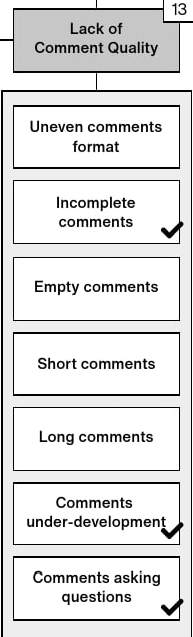
\includegraphics[height=350pt]{figs/goal-schema.PNG}
	\captionsetup{justification=centering}
	\caption{Comment categories the tool must be able to identify.}
	\label{fig:goal-schema}
\end{figure}

\noindent We began with simpler detections, such as identifying empty comments and comments that posed questions. Established rules were applied to determine if a comment was empty or contained either direct or implied questions.

\noindent Next, we tackled short and long comments. To achieve this, we utilized the \href{https://www.nltk.org/}{Natural Language Toolkit (NLTK)}, a comprehensive suite for natural language processing. By tokenizing each comment, we measured its length to classify it as either too short or overly long.

\noindent For comments under development, we employed pattern recognition techniques. We incorporated technical keywords and common phrases used during development to detect these comments.

\noindent The detection of incomplete comments and uneven comments format was refined through an iterative trial-and-error process, manually verifying results at each step. For incomplete comments, we initially performed a syntactic analysis to ensure the comments adhered to basic rules of English sentence structure. Subsequently, we built a classification system to categorize comments as single-line, multi-line, or documentation. For documentation comments, we verified consistency between the number of parameters in the comment and the corresponding source code, along with matching return types. Additionally, we introduced checks for single-line and multi-line comments to identify nonsensical or "gibberish" content, hence marking those that lacked clarity or coherence as incomplete.

\noindent Finally, for detecting uneven formatting, we flagged comments with irregular indentation, spacing, or annotation tag misuse, tailored to the programming language in use. This ensured that comments maintained proper structure, readability, and compliance with language-specific conventions.

\section{Logic Construction}

\begin{figure}[ht]
	\centering\includegraphics[width=400pt]{figs/whole-architecture.PNG}
	\captionsetup{justification=centering}
	\caption{General view on the tool's architecture.}
	\label{fig:whole-architecture}
\end{figure}

\noindent Let's discuss the architecture of our tool, which is organized into multiple layers. To provide clarity, we'll start with the foundational elements.

\begin{figure}[ht]
	\centering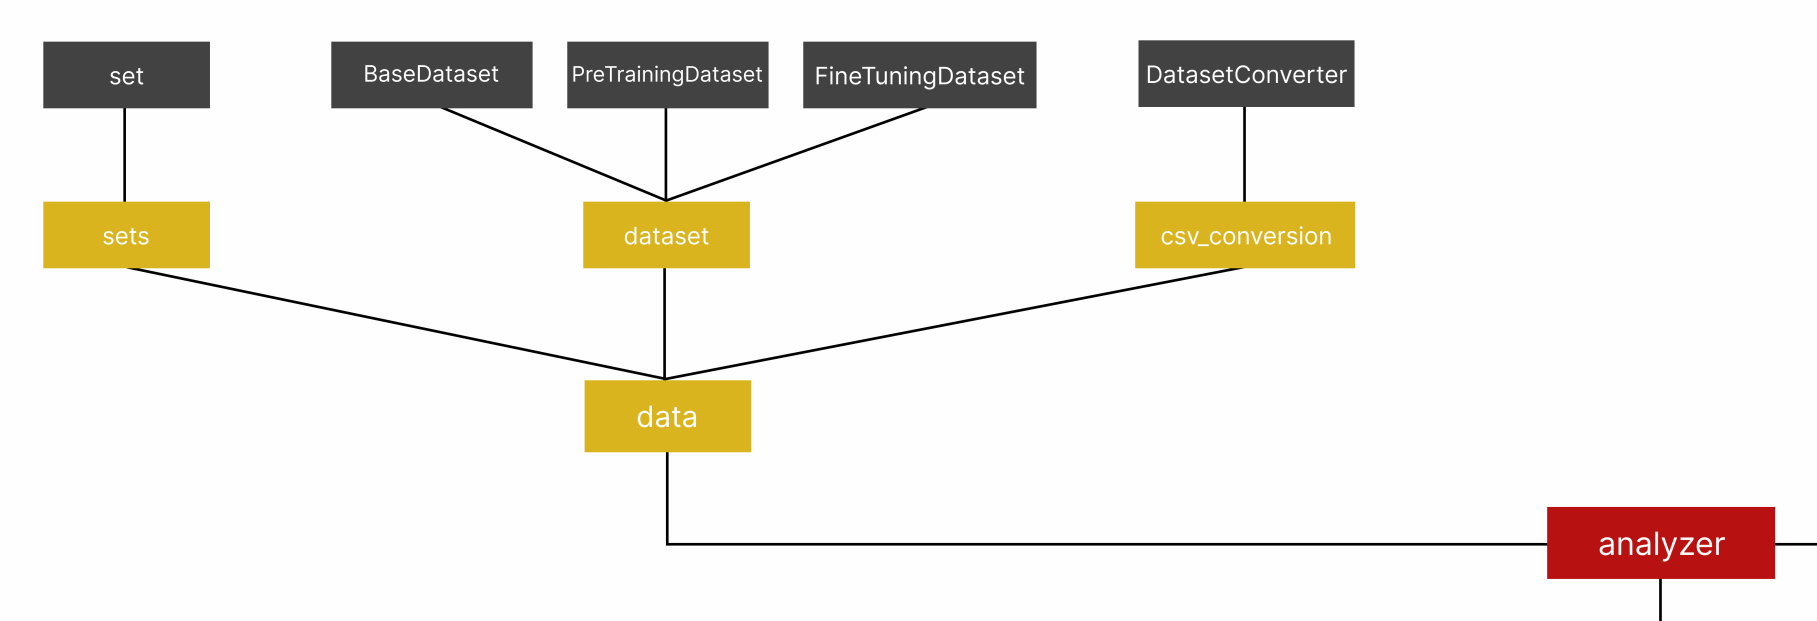
\includegraphics[width=400pt]{figs/zoom-data.PNG}
	\captionsetup{justification=centering}
	\caption{Zoom on the tool's data package.}
	\label{fig:zoom-data}
\end{figure}

\noindent The "data" package consists of three sub-packages:
	\begin{enumerate}
		\item \textbf{sets}: this sub-package contains the 'set' class, which defines the supported dataset file formats that our tool can read. The supported file extensions include \textit{.csv}, \textit{.tsv}, \textit{.json}, and \textit{.jsonl}.
		\item \textbf{dataset}: this sub-package contains several key classes:
			\begin{enumerate}
				\item \textbf{BaseDataset}: it provides a common interface for loading and working with various datasets, such as training, validation, and test sets.
				\item \textbf{PreTrainingDataset}: inheriting from BaseDataset, this class is designed to handle datasets specifically for pre-training models.
				\item \textbf{FineTuningDataset}: also inheriting from BaseDataset, this class is used for managing datasets in fine-tuning tasks.
			\end{enumerate}
		Both the \textit{PreTrainingDataset} and \textit{FineTuningDataset} classes default to the 'train' dataset if a specific set is not explicitly defined.
		\item \textbf{csv\_conversion}: this sub-package includes the \textit{DatasetConverter} class, which is used in cases where dataset format conversion is necessary.
	\end{enumerate}
	
\begin{figure}[ht]
	\centering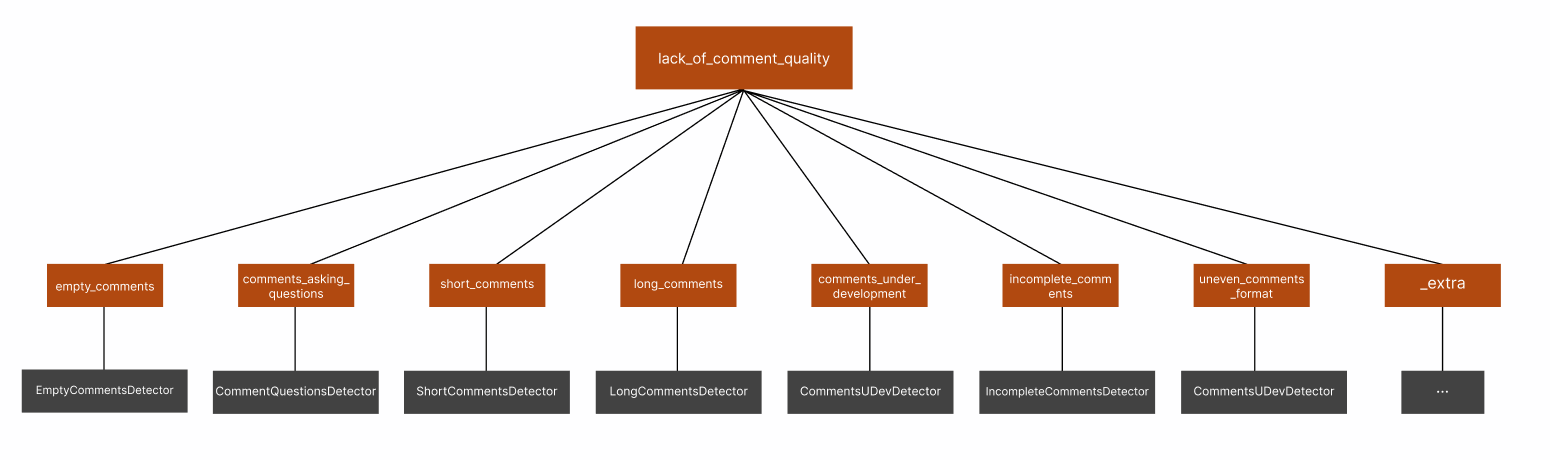
\includegraphics[width=465pt]{figs/zoom-cmsquality.PNG}
	\captionsetup{justification=centering}
	\caption{Zoom on lack of comments quality package.}
	\label{fig:zoom-cmsquality}
\end{figure}
	
\noindent The "smells" package contains our various detectors. I'm going to focus only on the "lack\_of\_comment\_quality" sub-package as the others are not part of this work.

\noindent Let’s begin with the "extra" sub-package, which might sound like an add-on, but contains essential components without which our tool wouldn't function.

\begin{figure}[ht]
	\centering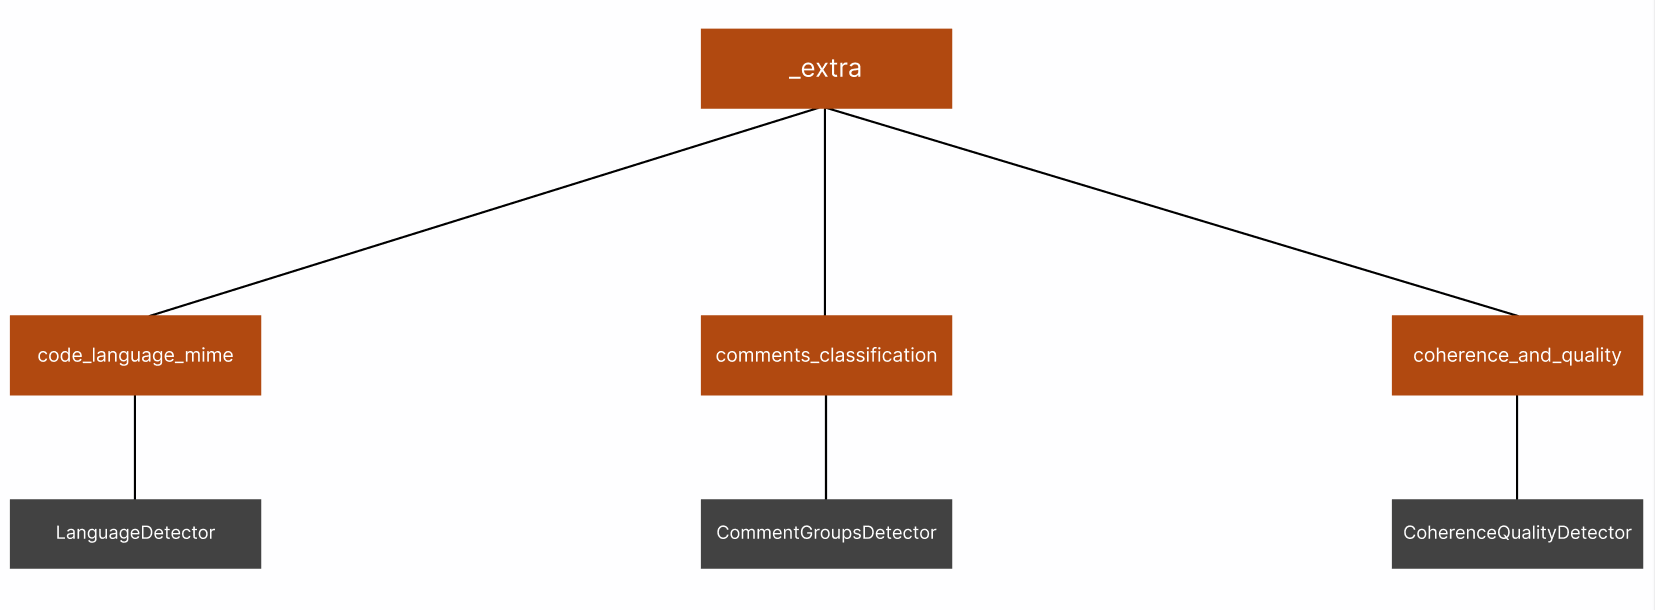
\includegraphics[width=400pt]{figs/zoom-extra.PNG}
	\captionsetup{justification=centering}
	\caption{Zoom on extra sub-package.}
	\label{fig:zoom-extra}
\end{figure}

\noindent Initially, we aimed for the tool to be language-agnostic, meaning it would work with all programming languages. While this is true for some detectors, it’s not feasible for all. As a result, we introduced a programming language detector, represented by the "code\_language\_mime" sub-package and its corresponding \textit{LanguageDetector} class. This class uses the \href{https://github.com/jossef/guesslang}{guesslang} library to identify the programming language used in a dataset and maps it to its MIME type.

\noindent The \textit{CommentGroupsDetector} class, located in the "comments\_classification" sub-package, scans all comments in the input database and categorizes them as single-line, multi-line, or documentation comments. This classification is crucial for enabling the incomplete comments detector and the uneven comments format detector to function correctly.

\noindent An additional detector, the \textit{CoherenceQualityDetector}, resides in the 

\noindent "coherence\_and\_quality" sub-package. This detector was developed while researching comment completeness, but it doesn’t strictly relate to incomplete comments, so it was placed in a separate package. The detector evaluates comments based on the following criteria:
	\begin{itemize}
		\item \textbf{Language (L)}: Ensures the comment is not written in a mix of different languages.
		\item \textbf{Clarity (C)}: Uses NLP techniques to assess the readability of the comment.
		\item \textbf{Relevance (R)}: Verifies that the comment accurately describes the specific code constructs it’s meant to explain.
		\item \textbf{Brevity (B)}: Checks if the comment avoids unnecessary repetition or wordiness.
		\item \textbf{Context (X)}: Determines whether the comment provides sufficient explanation for understanding the code.
	\end{itemize}
If a comment meets all these criteria, it is considered coherent. Otherwise, it is flagged as incoherent.

\noindent Let me now explain the "examples" package before listing the heuristics for the main smell detectors in the next paragraph.

\begin{figure}[ht]
	\centering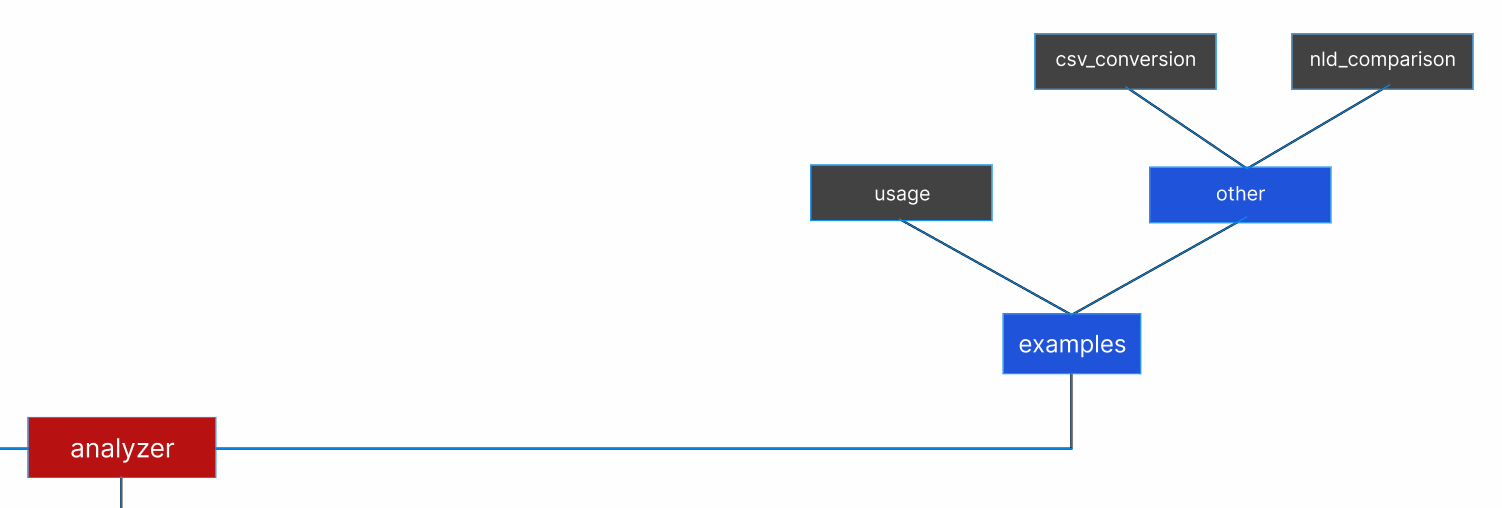
\includegraphics[width=400pt]{figs/zoom-examples.PNG}
	\captionsetup{justification=centering}
	\caption{Zoom on examples sub-package.}
	\label{fig:zoom-examples}
\end{figure}

\noindent The "examples" package contains the execution scripts for our tool. The key script is "example\_usage", which serves as the main file. This script loads the input dataset and sample, runs the desired detectors, and collects the results, returning a complete list of findings once the analysis is finished.

\noindent Within the "other" sub-package, there are two additional scripts:
	\begin{itemize}
		\item \textbf{example\_csv\_conversion}: this script uses the similarly named sub-package in "data" to convert raw datasets into a more readable format for the tool.
		\item \textbf{example\_nld\_comparison}: this script stems from a detailed study comparing the speed and accuracy of two NLP libraries, \href{https://spacy.io/}{\textit{spaCy}} and \href{https://fasttext.cc/}{\textit{fastText}}, for natural language detection. In our tool, language detection is essential for incomplete comment detection, as we first check whether a sentence is written in English. To evaluate the two libraries, we created a dictionary with words from eight different languages, then shuffled and combined them to generate a sample of 3,000 groups of sentences, where each is written in a different language. Both libraries successfully detected all languages, but spaCy took 99.51 seconds to complete, while fastText only required 24.25 seconds. Given its significantly superior speed, we opted for \textit{fastText} for natural language detection in our tool.
	\end{itemize}
	
\section{Heuristics Used}
We're now going to list all heuristics for each category from lack of comments quality.
In all cases:

\noindent Let \textit{C} represent a code block to be analyzed.

\noindent Let \textit{M} represent the MIME type (format) of the code block.

\noindent Let \textit{extract(C, M)} represent the function that extracts comments from \textit{C} based on MIME type \textit{M}.

\noindent Let \textit{comment(i)} represent the i-th comment in the extracted list of comments from \textit{C}.

\noindent Let \textit{text(i)} represent the text of the i-th comment.

\subsection{Empty Comments}
\noindent Let's define the empty comment condition as isEmpty\textit{(i)}, where: 
\begin{equation*}
	\textbf{isEmpty}(i) = \begin{cases}
		1, & \text{if } \text{ strip(text\textit{(i)}) = ""} \\
		0, & \text{ otherwise}
	\end{cases}
\end{equation*}
where \textit{strip(text(i))} removes all leading and trailing whitespace from the comment.

\noindent We define the function \textit{F(C, M)} that evaluates if the code block \textit{C} contains empty comments based on the MIME type \textit{M}:
\begin{equation*}
	F(C, M) = \begin{cases}
		1, & \text{if } \exists i \text{ such that } \text{isEmpty}(i) = 1 \text{ for any comment } i \in \text{extract}(C, M) \\
		0, & \text{ otherwise}
	\end{cases}
\end{equation*}

\subsection{Comments Asking Questions}
Let's define the set of interrogative phrases as:
\begin{equation*}
	I = \text{\{"why", "how", "what is", "what\\'s", "where\\'s", "where is", "where are", "how long"\}}
\end{equation*}

\noindent Then let's define the question condition as isQuestion\textit{(i)}, where:
\begin{equation*}
	\textbf{isQuestion}(i) = \begin{cases}
		1, & \text{if } \text{text}(i) \text{.endswith("?")} \vee \text{text}(i) \text{.startswith}(I) \\
		0, & \text{ otherwise}
	\end{cases}
\end{equation*}

\noindent We define the function \textit{F(C, M)} that evaluates if the code block \textit{C} contains any questions based on the MIME type \textit{M}:
\begin{equation*}
	F(C, M) = \begin{cases}
		1, & \text{if } \exists i \text{ such that } \text{isQuestion}(i) = 1 \text{ for any comment } i \in \text{extract}(C, M) \\
		0, & \text{ otherwise}
	\end{cases}
\end{equation*}

\subsection{Short Comments}
Let T\textit{(i)} = tokenize(text\textit{(i)}) be the list of tokens in the i-th comment.

\noindent Let's define a threshold for short comments as k = 5 (maximum number of tokens).

\noindent Let's define the short comments condition as isShort\textit{(i)}, where:
\begin{equation*}
	\textbf{isShort}(i) = \begin{cases}
		1, & \text{if } \mathrm{|T|}_{i} \le k \\
		0, & \text{ otherwise}
	\end{cases}
	
	\noindent \text{where} \mathrm{|T|}_{i} \text{ represents the number of tokens in the i-th comment.}
\end{equation*}

\noindent We define the function \textit{F(C, M)} that evaluates if the code block \textit{C} contains any short comments based on the MIME type \textit{M}:
\begin{equation*}
	F(C, M) = \begin{cases}
		1, & \text{if } \exists i \text{ such that } \text{isShort}(i) = 1 \text{ for any comment } i \in \text{extract}(C, M) \\
		0, & \text{ otherwise}
	\end{cases}
\end{equation*}

\subsection{Long Comments}
The heuristic is similar to that used for short comments, but in the first case, the comparison is reversed.
It's inspired by the work of \textit{Steidl et al.} \cite{steidl2013}, but our approach uses tokens rather than words.

\noindent Let's define a threshold for long comments as k = 30 (minimum number of tokens).

\noindent Let's define the long comments condition as isLong\textit{(i)}, where:
\begin{equation*}
	\textbf{isLong}(i) = \begin{cases}
		1, & \text{if } \mathrm{|T|}_{i} \ge k \\
		0, & \text{ otherwise}
	\end{cases}
	
	\noindent \text{where} \mathrm{|T|}_{i} \text{ represents the number of tokens in the i-th comment.}
\end{equation*}

\begin{equation*}
	F(C, M) = \begin{cases}
		1, & \text{if } \exists i \text{ such that } \text{isLong}(i) = 1 \text{ for any comment } i \in \text{extract}(C, M) \\
		0, & \text{ otherwise}
	\end{cases}
\end{equation*}

\subsection{Comments Under Development}
This heuristic is inspired by the work of \textit{Shi et al.} \cite{buildingRock}.

\noindent Let's define the following sets of keywords:
	\begin{itemize}
		\item \textit{P} = placeholder keywords, e.g., "Description of the Method", "Logic goes here".
		\item \textit{N} = temporary notes, e.g., "Add more info here", "Temporary fix for issue".
		\item \textit{D} = vague descriptions, e.g., "To be documented", "Work in progress".
		\item \textit{R} = redundant keys, e.g., "Opens a file", "Calls the method".
		\item Let $\mathrm{R}_{M}$ represent a set of MIME-type specific patterns to detect commented methods (e.g., method definitions in Java, Python, etc.).
	\end{itemize}
	
\noindent Let\begin{math*}
	regexMatch(\textit{i, P, N, D, R, } \mathrm{R}_{M})
\end{math*} be a function that checks whether any of the patterns defined by \begin{math*}\textit{P, N, D, R, } \mathrm{R}_{M} \end{math*} match the comment text \textit{text(i)}.

\noindent Let's define the under development condition as isUnderDev\textit{(i)}, where:
\begin{equation*}
	\textbf{isUnderDev}(i) = \begin{cases}
		1, & \text{if } \text{regexMatch(i, P, N, D, R, }  \mathrm{R}_{M}) = 1 \\
		0, & \text{ otherwise}
	\end{cases}
\end{equation*}

\noindent We define the function \textit{F(C, M)} that evaluates if the code block \textit{C} contains any comments indicative of being "under development" based on the MIME type \textit{M}:
\begin{equation*}
	F(C, M) = \begin{cases}
		1, & \text{if } \exists i \text{ such that } \text{isUnderDev}(i) = 1 \text{ for any comment } i \in \text{extract}(C, M) \\
		0, & \text{ otherwise}
	\end{cases}
\end{equation*}

\subsection{Incomplete Comments}
Let \textit{SML} represent groups of comments classified by \textit{CommentGroupsDetector} into single-line or multi-line.

\noindent Let \textit{DOC} represent the group of comments classified as documentation by \textit{CommentGroupsDetector}.

\noindent Let's assume we're able to detect different types of comment formats (e.g., \textit{Google}, \textit{NumPy}, \textit{ReST}, \textit{epytext}, \textit{Javadoc}) based on the detected structure of comments and the programming language.

\noindent For single-line and multi-line comments, first we have to check whether a comment is written in English.
\begin{equation*}
	\mathrm{F}_{english}(comment) = \begin{cases}
		1, & \text{if the comment} \in \textit{SML } \wedge \text{ is classified as English} \\
		0, & \text{if the comment} \in \textit{SML } \text{ but is in a different language}
	\end{cases}
\end{equation*}

\noindent Then, we check the syntactic completeness of a comment by verifying if each sentence contains a subject and a predicate, assuming the comment $\in$ \textit{SML}.
\begin{equation*}
	\mathrm{F}_{syntax}(comment) = \begin{cases}
		1, & \text{if  } \exists \text{sentence} \in \text{comment syntactically incomplete} \\
		0, & \text{if all sentences are complete}
	\end{cases}
\end{equation*}

\noindent Lastly, we evaluate whether a comment, assumed $\in$ \textit{SML}, is gibberish using a pre-trained model \cite{gibberishDetector} that classifies comments into various categories.
\begin{equation*}
	\mathrm{F}_{gibberish}(comment) = \begin{cases}
		1, & \text{if  } \exists \text{sentence} \in \text{comment classified as gibberish} \\
		0, & \text{if all sentences are clean}
	\end{cases}
\end{equation*}

\noindent For documentation comments, we must check if a comment is missing any critical part in annotation tags (wrong number of params, lack of return type) compared to the code block it refers to.

\noindent Let $\mathrm{P}_{comment}$ represent the number of @param annotations in the comment, assuming comment $\in$ \textit{DOC}.

\noindent Let $\mathrm{R}_{comment}$ represent the number of @return annotations in the comment (which can be only 0 or 1), assuming comment $\in$ \textit{DOC}.

\noindent We check the number of parameters in the function signature.
\begin{equation*}
	\mathrm{F}_{params}(C) = \begin{cases}
		n, & \text{if the function has parameters} \\
		0, & \text{if no parameters exist}
	\end{cases}
\end{equation*}

\noindent Then, we check the return type in the function signature.
\begin{equation*}
	\mathrm{F}_{return}(C) = \begin{cases}
		1, & \text{if it returns a value other than void
		} \\
		0, & \text{if it returns void or no return type is found}
	\end{cases}
\end{equation*}

\noindent To conclude we can say that, for a single-line or multi-line comment to be incomplete, the following conditions must be met:
	\begin{enumerate}
		\item The comment is in English.
		\item The comment is syntactically incomplete.
		\item The comment contains gibberish.
	\end{enumerate}
	
\noindent Thus, the overall incompleteness function for single-line or multi-line comments $\mathrm{F}_{incomplete}^{\textit{ SML}}$ can be expressed as:
\begin{equation*}
	\mathrm{F}_{incomplete}^{\textit{ SML}} = \begin{cases}
		1, & \text{if } \mathrm{F}_{english}(comment) = 1 \wedge \mathrm{F}_{syntax}(comment) = 1 \wedge \mathrm{F}_{gibberish}(comment) = 1 \\
		0, & \text{otherwise}
	\end{cases}
\end{equation*}

\noindent For a documentation comment to be incomplete, it means there is either a mismatch between the number of \textit{@param} annotations and the actual number of parameters, or a mismatch between the presence of a \textit{@return} annotation and whether the function actually returns a value.

\noindent This implies that the incompleteness function for documentation comments $\mathrm{F}_{incomplete}^{\textit{ DOC}}$ can be expressed as:
\begin{equation*}
	\mathrm{F}_{incomplete}^{\textit{ DOC}} = \begin{cases}
		1, & \text{if } \mathrm{P}_{comment} \ne \mathrm{F}_{params}(C) \\
		1, & \text{if } \mathrm{R}_{comment} = 1 \wedge \mathrm{F}_{return}(C) = 0 \\
		1, & \text{if } \mathrm{R}_{comment} = 0 \wedge \mathrm{F}_{return}(C) = 1 \\
		0, & \text{otherwise}
	\end{cases}
\end{equation*}

\subsection{Uneven Comments Format}
Let \textit{SL} be the group of single-line comments, \textit{ML} the group of multi-line comments and \textit{DOC} the group of documentation comments.

\noindent Let \textit{SF} be the single-line way of comment formatting (e.g, // in \textit{Java}, # in \textit{Python}).

\noindent Let \textit{MF} be the multi-line way of comment formatting (e.g, /* or /** in \textit{Java}, ''' or """ in \texit{Python})

\noindent Let \textit{TAGS} be an array of commonly used HTML tags in Javadoc comments.

\noindent Let \textit{S} be a sentence $\in$ comment.

\noindent Let spaces\textit{(S)} represent the number of spaces in that sentence.

\noindent Let \textit{K} be the maximum number of spaces allowed per sentence.

\noindent We have a function that checks whether there are too many spaces (more than \textit{K} consecutive) in any sentence from the comment, which could indicate indentation issues.
\begin{equation*}
	\mathrm{F}_{spacing}(comment) = \begin{cases}
		1, & \text{if } \exists S \in comment : spaces(S) > K \\
		0, & \text{otherwise}
	\end{cases}
\end{equation*}

\noindent Single-line and multi-line comments shouldn't contain any HTML tags, as they are treated as plain text.
Assuming comment $\in$ \textit{SL} $\vee$ comment $\in$ \textit{ML}:
\begin{equation*}
	hasTags(comment) = \begin{cases}
		1, & \text{if } \exists T \subset TAGS : T \in comment \\
		0, & \text{otherwise}
	\end{cases}
\end{equation*}

\noindent For a single-line comment to be uneven, we check the number of spaces or if it matches the multi-line format.
\begin{equation*}
	\mathrm{F}_{uneven}^{\textit{ SL}}(comment, MF) = \begin{cases}
		1, & \text{if } \mathrm{F}_{spacing} = 1 \vee hasTags(comment) = 1 \vee match(comment, MF) \\
		0, & \text{otherwise}
	\end{cases}
\end{equation*}

\noindent For a multi-line comment to be uneven, we do the opposite.
\begin{equation*}
	\mathrm{F}_{uneven}^{\textit{ ML}}(comment, SF) = \begin{cases}
		1, & \text{if } \mathrm{F}_{spacing} = 1 \vee hasTags(comment) = 1 \vee match(comment, SF) \\
		0, & \text{otherwise}
	\end{cases}
\end{equation*}

\noindent For documentation comments, we have a function that checks for irregularities in the use of annotation tags (e.g, wrong indentation, empty annotation, wrong token after annotation, ends with annotation). In particular, if the annotation is \textit{@author} and the following token is a verb, it makes no sense. If the annotation is followed by a redundant token (e.g, @return nothing), it should be avoided.

\noindent Let \textit{RDT} be an array of possible redundant words after an annotation (e.g, author, param, nothing, none, void).
Assume comment $\in$ \textit{DOC}, and the current token is an annotation.
\begin{equation*}
	\mathrm{F}_{irr}^{\textit{ DOC}}(comment) = \begin{cases}
		1, & \text{if } \text{token} = \textit{'@author'} \wedge \text{token\textit{.next}} \in \text{'VERB'} \\
		1, & \text{if } isSpace(token.next) = 1 \wedge \mathrm{F}_{spacing} = 1 \\
		1, & \text{if } isEmpty(token.next) = 1 \\
		1, & \text{if } token.next \in RDT \\
		0, & \text{otherwise}
	\end{cases}
\end{equation*}

%% Chapter 4

\chapter{Empirical Study} % Main chapter title

\label{Chapter4}

%----------------------------------------------------------------------------------------

Our goal is to develop a tool capable of detecting lack of quality in comments from large code-related datasets with the highest level of precision possible. In the field of code comment analysis, researchers have explored various metrics and models to evaluate comment quality, categorizing comments in programming languages like \textit{Java} and \textit{Python}. However, these efforts are limited to only a few languages.
Looking forward, it is likely that researchers will aim to extend these models to cover a broader range of programming languages while improving the accuracy of their assessments. Future works will also increasingly incorporate artificial intelligence (AI) and machine learning techniques, which rely heavily on vast datasets to function effectively. As these approaches evolve, access to high-quality datasets with a large number of diverse instances will become essential.
To achieve this, automating the retrieval of such instances is crucial. This will enable the collection of comprehensive datasets that not only support the refinement of existing comment quality models but also facilitate the development of more robust and versatile tools capable of analyzing code comments across multiple programming languages with precision and scalability.

\section{Study Design}
The goal of this study is to understand to what extent the proposed heuristics allow to detect true comments lacking quality. Our study is steered by the following research
question:
\begin{large}
	\begin{Center}
		\textbf{RQ:} With which level of precision is it possible to automatically recognize poor-quality comments in large code-related datasets?
	\end{Center}
\end{large}

\subsection{Data Collection}
In order to validate our heuristic, we concentrated on two datasets: CSN \cite{CSN} and AUGER \cite{AUGER}, both of which are vastly utilized in literature.

\noindent CSN is a large-scale dataset designed to facilitate semantic code search, which is the process of retrieving relevant code snippets based on natural language queries.
The dataset includes over 6 million functions from six programming languages, but our subset focuses solely on \textit{Java}.

\noindent AUGER is designed for generating automated review comments in code reviews, using the Text-to-Text Transfer Transformer (T5) pre-trained model. The dataset includes data collected from 11 notable Java open-source projects on GitHub.

\noindent We selected two case-study samples of 384 instances from each dataset.

\subsection{Data Analysis}
We manually analyzed the comments from both samples, assigning a value of 0 when the comment did not meet a detection criteria, and 1 when it did. In ambiguous cases, we defaulted to 0. 
For the purpose of validating our heuristic, we compared its results against our manual annotations, using the metrics of accuracy, precision, recall, and f1score for each criteria. These metrics were computed with the following formulas:
\begin{equation*}
	accuracy = \frac{TP + TN}{TP + TN + FP + FN}		
\end{equation*}
\begin{equation*}
	precision = \frac{TP}{TP + FP}
\end{equation*}
\begin{equation*}
	recall = \frac{TP}{TP + FN}
\end{equation*}
\begin{equation*}
	f1score = 2 \times \frac{precision \times recall}{precision + recall}
\end{equation*}
With the term TP we indicate those comments that are caught by our heuristics in one of the detection criteria. With the term TN we indicate those comments that are not caughty by our heuristics in one or any of the detection criteria. With the term FP we indicate those comments that are detected by our heuristic in one of the criteria but actually shouldn't. With the term FN we indicate those comments that aren't detected by our heuristic in one or any of the criteria but actually should.

\section{Study Results}
TODO

\section{Threats to Validity}
This section discusses the threats to validity of this heuristic. Specifically, (I) construction validity regarding manual testing, (II) internal validity regarding possible impairment of results and (III) external validity regarding the dataset.

\subsection{Construct Validity}
We have detailed the logic behind our heuristics and described the validation process used to evaluate their effectiveness by extracting key metrics. The heuristics were tested on 384 instances from the \textit{CSN} dataset and 100 instances from \textit{AUGER}. This process involved manually labeling each comment, meaning that any misinterpretation of the comments could potentially compromise the validity of the results. To mitigate this risk, we thoroughly reviewed and examined all comments multiple times to ensure accuracy and reduce the likelihood of errors in interpretation.

\subsection{Internal Validity}
To address the research question, we developed heuristics grounded in our knowledge of the domain. This approach involved incorporating our own insights and patterns related to comment analysis, which may have introduced some subjectivity, particularly in the more complex detectors, such as those for incomplete comments and uneven comment formatting. However, we aimed to select rules that are broadly applicable and objective, while maintaining a disciplined approach to minimize subjectivity and ensure consistency in our criteria.

\subsection{External Validity}
TODO
 
%% Chapter 5

\chapter{Conclusion and Future Work} % Main chapter title

\label{Chapter5}

%----------------------------------------------------------------------------------------

\section{Conclusion}
We explored the critical role of code comment analysis in improving software maintainability, readability, and overall quality. Many analyses have been made to study the quality of comments, yet the majority of them focus on key specifics, one or two study scopes. We aim for more general approaches that allow to study comments quality from a variety of points of view. As such, we presented several criteria that help us divide comments in different categories, and for each category we have developed an appropriate heuristic. By leveraging natural language processing (NLP) and machine learning techniques, we tested our approach using real-world datasets. In fact, as part of our validation process, we applied them on two sets of 384 instances each from CSN and AUGER, obtaining as a result a score of precision of (TODO) for CSN and (TODO) for AUGER.

\section{Future Work}
This work has laid the foundation for numerous future advancements in code comment analysis. The categorizations and heuristics developed can serve as valuable resources for building machine learning models that enhance detection accuracy and extend the analysis beyond the initial scope. Future research can explore additional categories and aspects of comments that can be inferred, while also expanding the tool's applicability to a wider range of programming languages.

\noindent One of our ongoing goals is to further minimize false positives by refining the heuristics to be more precise and objective, ensuring that as few relevant instances as possible are excluded. Ultimately, this work contributes to the expanding field of automated quality assurance, helping to bridge the gap between human-readable comments and machine-driven analysis, and paving the way for more maintainable and robust codebases in the future. 

%----------------------------------------------------------------------------------------
%	THESIS CONTENT - APPENDICES
%----------------------------------------------------------------------------------------

%\appendix % Cue to tell LaTeX that the following "chapters" are Appendices

% Include the appendices of the thesis as separate files from the Appendices folder
% Uncomment the lines as you write the Appendices

%\include{Appendices/AppendixA}
%\include{Appendices/AppendixB}

%----------------------------------------------------------------------------------------
%	BIBLIOGRAPHY
%----------------------------------------------------------------------------------------
\nocite{*}

\renewcommand{\mkbibnamefirst}[1]{\textsc{#1}}
\renewcommand{\mkbibnamelast}[1]{\textsc{#1}}
\renewcommand{\mkbibnameprefix}[1]{\textsc{#1}}
\renewcommand{\mkbibnameaffix}[1]{\textsc{#1}}

\printbibliography[heading=bibintoc]

%----------------------------------------------------------------------------------------


\newpage\thispagestyle{empty}
\vspace*{0.2\textheight}

%\noindent\enquote{\itshape ...}\bigbreak

\end{document}